\documentclass{report}

\usepackage[pdftex,
  colorlinks=true,
  pdfstartview=FitV,
  linkcolor=blue,
  citecolor=blue,
  urlcolor=blue]{hyperref}
\usepackage{xspace}
\usepackage{geometry}
\geometry{a4paper}
\usepackage{indentfirst}
\usepackage[francais]{babel}
\usepackage[latin1]{inputenc}
\usepackage[dvips]{graphicx}

\newcommand{\visidia}{ViSiDiA\xspace}
\newcommand{\dossier}[1]{$#1$}
\newcommand{\classe}[1]{$#1$}
\newcommand{\methode}[1]{$#1$}

\title{Mode d'emploi pour \visidia et les agents mobiles}
\author{L'�quipe PFA \visidia 2006}
\date{Avril 2006}

\begin{document}
\maketitle
\tableofcontents


% Simu Agent mobile
%   Ajouter 1 agent
%      Via API
%        - manu
%        - placeur
%      Via regles de reecriture
%   Edition WhiteBoards
%     WB Agent
%     WB Sommet
%       - def
%       - specif
%   Execution simulation
%     pulse stop pause
%   Statistiques
%       
% Programmation      
%   Agent
%   Agent Sync
%   Mover
%   Placeur
%   Stats

\chapter{Objet}

Ce  document est un  aper�u de  l'utilisation  de
\visidia avec  les agents mobiles.  Nous consid�rerons que  le lecteur
ma�trise d�j�  \visidia et  que l'environnement de  d�veloppement Java
est d�j� install� et configur�.\\

Dans  un premier  temps, nous  t�l�chargerons la  branche  de \visidia
concernant  les  agents  et  compilerons  l'ensemble.   Ensuite,  nous
d�crirons en  profondeur l'interface li�e � la  simulation des agents.
Enfin, nous pr�senterons l'API  des agents et d�taillerons la proc�dure
pour  en cr�er  de nouveaux,  ainsi que  les m�thodes  pour  cr�er ses
propres modules  de d�placement, de placement initial  d'agents sur le
graphe et de statistiques.


%%% Local Variables: 
%%% mode: latex
%%% TeX-master: "main"
%%% coding: latin-1
%%% TeX-PDF-mode: t
%%% End: 

\chapter{Installer et lancer \visidia}

Il existe  deux techniques pour  r�cup�rer \visidia dot� de  la partie
agents mobiles.  Soit vous  utilisez une version suppos�e stable, soit
vous r�cup�rez une version de d�veloppement. 


\section{R�cup�rer la version stable}

Pour   r�cup�rer    la   version    stable,   allez   sur    le   site
\url{https://developer.berlios.de/projects/visidia/}. Au  milieu de la
page,  vous trouverez  une  section nomm�e  \og Derni�res r�visions  des
fichiers \fg. Cliquez  alors sur le lien t�l�chargement  et r�cup�rez le
fichier le plus r�cent. Enfin,  d�compressez le fichier � l'aide de la
commande :

\begin{verbatim}
$ tar xvfj lefichiertelecharge.tar.bz2
\end{verbatim}


\section{R�cup�rer la version en d�veloppement}

Pour disposer de la version  de d�veloppement, vous devez poss�der SVN
qui   est  un   rempla�ant   de   CVS  disponible   sur   le  site   :
\url{http://subversion.tigris.org/}.\\

Le gestionnaire de version SVN est compil� et disponible sous forme de
paquets pr�s � l'emploi pour la majorit� des distributions Linux. Sous
Windows,   TortoiseSVN   permet   de   travailler  sous   SVN   depuis
l'explorateur   de   fichiers.  Il   est   disponible   sur  le   site
\url{http://www.tortoisesvn.tigris.org/}.\\


Pour  t�l�charger la  version de  d�veloppement, utilisez  la commande
suivante :

\begin{verbatim}
$ svn checkout svn://svn.berlios.de/visidia/trunk/src visidia
\end{verbatim}

Cela va cr�er un r�pertoire \dossier{visidia} dans le dossier courant. 


\section{Compiler et lancer \visidia}

Pour compiler  \visidia, le  kit de d�veloppement  Java 5.0  doit �tre
install� et pr�sent dans votre PATH.  Il est disponible sur le site de
SUN   \url{http://java.sun.com/j2se/1.5.0/download.jsp}.\\   Pour   le
v�rifier :

\begin{verbatim}
$ javac -version
javac 1.5.0
$
\end{verbatim}

Placez-vous  dans  le  r�pertoire  \dossier{visidia} et  ex�cuter  les
commandes suivantes pour compiler puis pour lancer \visidia :

\begin{verbatim}
$ ./compile.sh
$ ./acompile.sh
$ ./visidia.sh
\end{verbatim}

La premi�re  ligne compile \visidia  et les
modules  comme les algorithmes,  les agents  etc.  La  deuxi�me lance
\visidia. Suivant votre installation,  vous pourriez avoir de nombreux
messages d'avertissements concernant les accents. Ces messages ne sont
pas bloquants, vous pouvez les ignorer.\\

Si tout  c'est bien pass�,  \visidia devrait �tre lanc�.  Vous devriez
voir l'application comme sur la figure \ref{fig:visidia}.

\begin{figure}[ht]
  \centering
  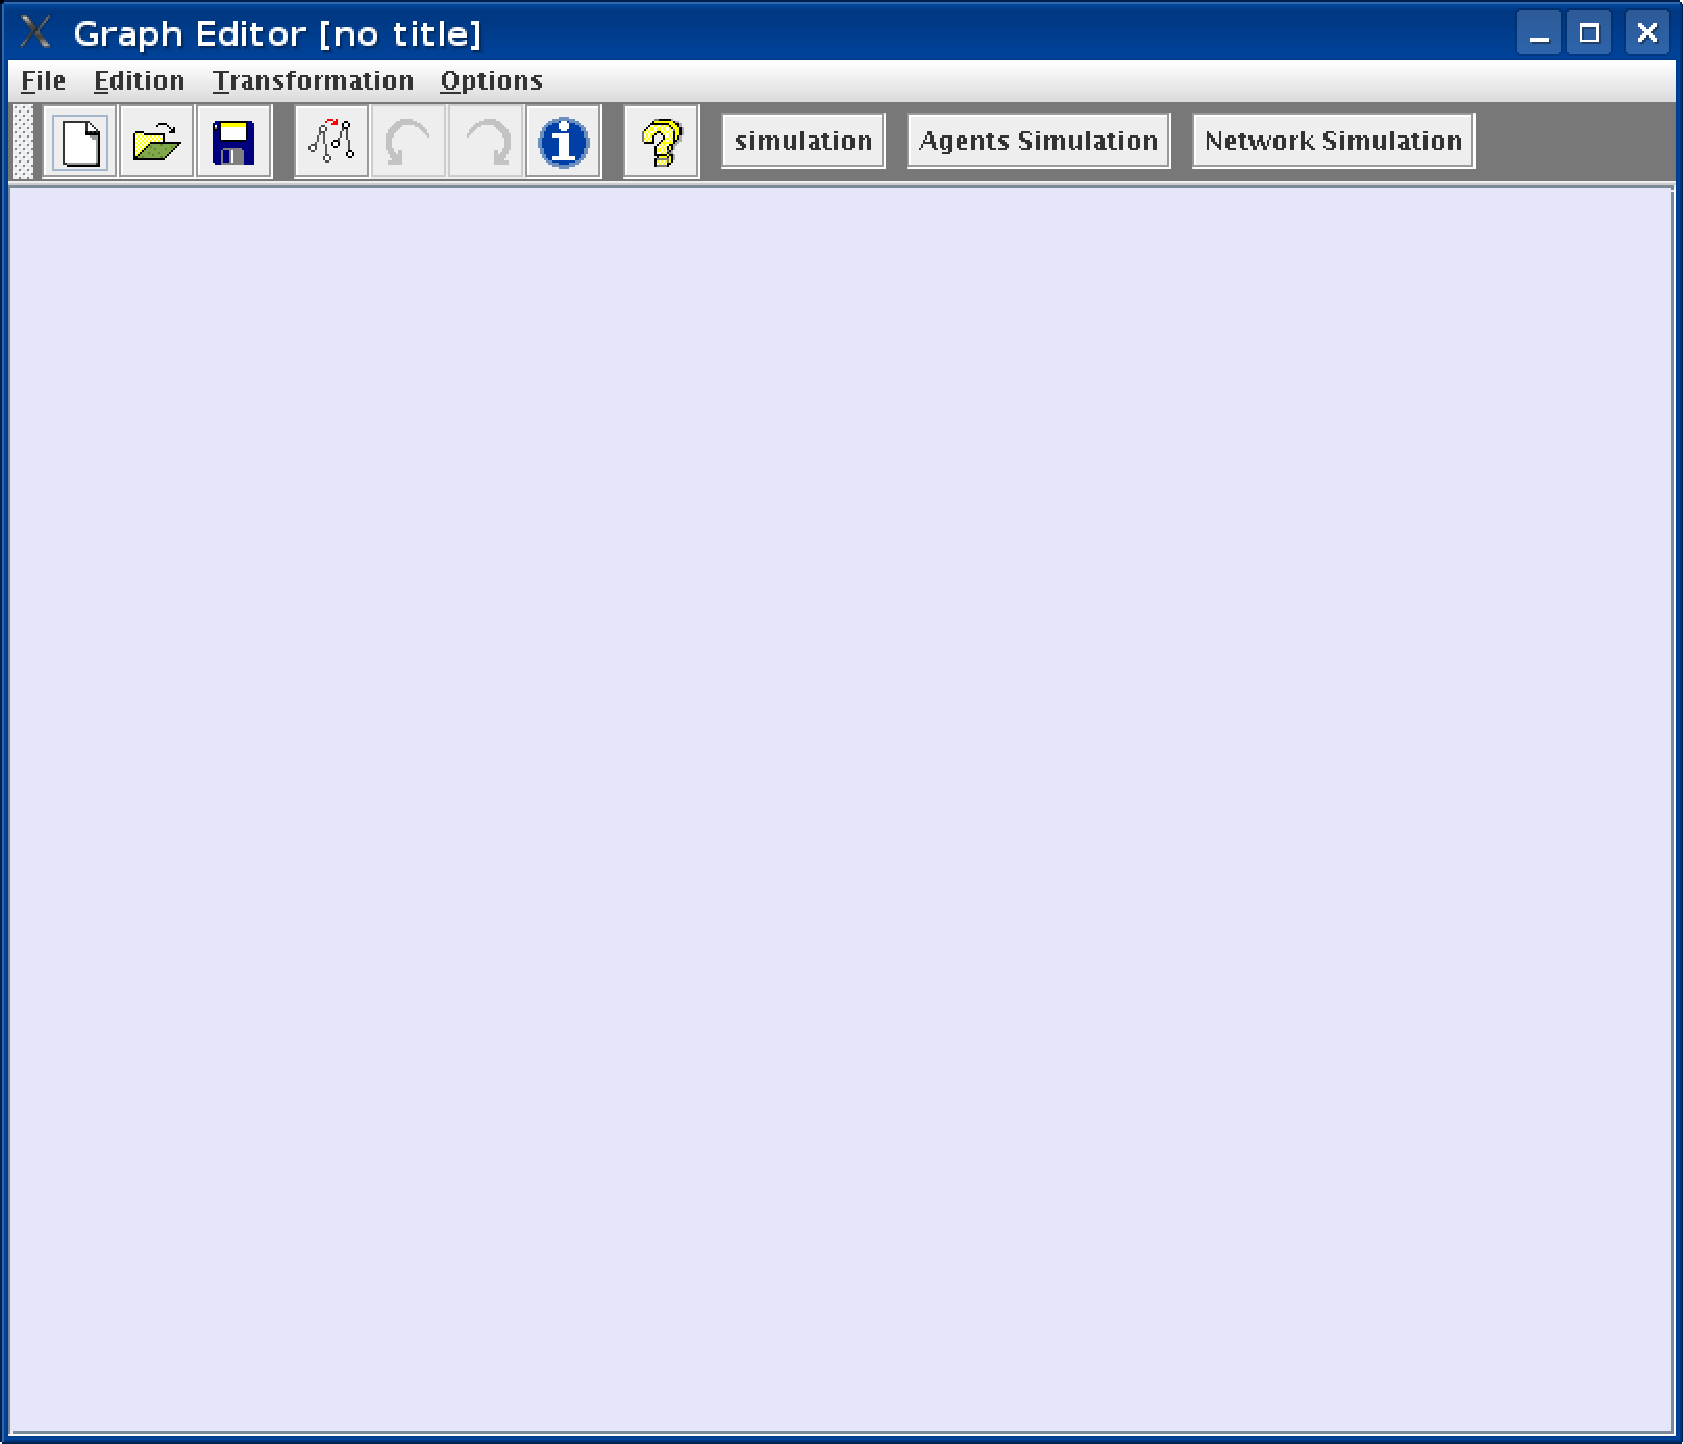
\includegraphics[width=10cm]{visidia.pdf}
  \caption{Lancement de \visidia}
  \label{fig:visidia}
\end{figure}

%%% Local Variables: 
%%% mode: latex
%%% TeX-master: "main"
%%% coding: latin-1
%%% TeX-PDF-mode: t
%%% End: 

\chapter{Creation d'un graphe}

Une fois \visidia lanc�, la fen�tre d'�dition de graphe appara�t :

Le graphe se construit � l'aide du clic gauche de la souris (cette
fonctionnalit� reste disponible lors de la simulation avec agents mobiles). Les
graphes peuvent �galement �tre sauvegard� gr�ce aux commandes \textbf{Save}
ou \textbf{Save as...} du menu \textbf{File}.

Dans le menu Transformation :
\begin{itemize}
\item \textbf{Complete} permet de transformer le graphe courant en un graphe complet.
\item \textbf{Delete edges} permet d'effacer les ar�tes du graphe.
\item \textbf{Change edges shape} permet de modifier la nature du graphe
  (orient� ou non orient� - les agents mobiles ne supportent que les
  graphes non-orient�).
\item \textbf{Change vertices shape} permet de modifier la nature des
  sommets du graphe.
\item \textbf{Vertex renumbering} permet de renum�roter les sommets du
  graphs.
\end{itemize}

Une fois le graphe cr��, il est possible de faire ex�cuter \visidia
selon trois mode :

\begin{itemize}
\item Simulation avec des messages en local : bouton \textbf{Simulation}
\item Simulation avec des messages avec r�partition des noeuds du
  graphe sur plusieurs machines : bouton \textbf{Network Simulation}
\item Simulation avec des agents mobiles en local : bouton \textbf{Agents Simulation}
\end{itemize}


%%% Local Variables: 
%%% mode: latex
%%% TeX-master: "main"
%%% coding: latin-1
%%% TeX-PDF-mode: t
%%% End: 

\chapter{Simulation avec des agents mobiles}

\section{Ajouter un ou des agents au graphe}

La  premi�re �tape de  la simulation  avec des  agents mobiles  est le
placement  d'agents sur  des sommets.  Pour effectuer  ceci, plusieurs
m�thodes peuvent �tre envisag�es :

\begin{itemize}

\item Le placement manuel

\item Le placement programm�

\item Les r�gles de r��critures

\end{itemize}

\subsection{Ajouter des agents �crits avec l'API}

Pour les agents �crits avec  l'API, s�lectionnez dans un premier temps
le(s) sommet(s)  sur le(s)quel(s) vous souhaitez ajouter  un agent. La
selection  se fait  avec un  clic  droit de  la souris  (si besoin  en
maintenant  la touche SHIFT  en cas  de s�lection  multiple).  Ensuite
utilisez  la commande \textbf{Add  Agent...}  du  menu \textbf{Agent}.
S�lectionnez  alors  le  type   d'agent  �  ajouter  en  s�lectionnant
l'algorithme   compil�  dans   la  boite   de  dialogue.    Pour  plus
d'information sur l'�criture d'algorithmes � l'aide de l'API, veuillez
vous r�f�rer � la section \emph{Programmer des agents avec l'API}.

\subsection{Ajouter des agents de fa�on programm�e}

Lancer    la    commande    \textbf{Place    Agents...}     du    menu
  \textbf{Agents}. Cette technique  de placement ne fonctionne qu'avec
  les algorithmes  compil�s avec  l'API, et permet  de placer  un type
  d'agent choisi de fa�on programm�e sur le graphe : par exemple, vous
  pourrez placer  un type d'agent sur  les sommets du  graphe avec une
  probabilit� de 1/2 pour chaque sommet.\\

Pour   programmer   votre   placeur,   r�ferez-vous   �   la   section
  \ref{sec:prog-placeur}


\subsection{Ajouter des agents d�finis avec des r�gles de r��critures}

Avec l'�criture de  code, il existe un autre  mod�le de repr�sentation
pour les algorithmes  distribu�s : les r�gles de  r��critures. Gr�ce �
ces r�gles,  un utilisateur peut litt�ralement  dessiner un algorithme
avec sa souris � l'int�rieur de \visidia et le valider pour suivre son
ex�cution  comme  s'il l'avait  �crit  en  Java.  Consultez la  figure
\ref{fig:existant-regles} pour un exemple de r�gle.

Vous avez deux possibilit�s pour vous servir des r�gles de r��critures
:

  \begin{itemize}

  \item Cr�er un nouveau jeu de r�gles de r��critures avec la commande
     \textbf{New relabeling system} du menu \textbf{Rules}.

  \item Ouvrir un jeu de r�gles de r��critures pr�c�demment sauvegard�
    avec la commande \textbf{Open rules...} du menu \textbf{Rules}.

  \end{itemize}

\begin{figure}[ht]
  \centering
  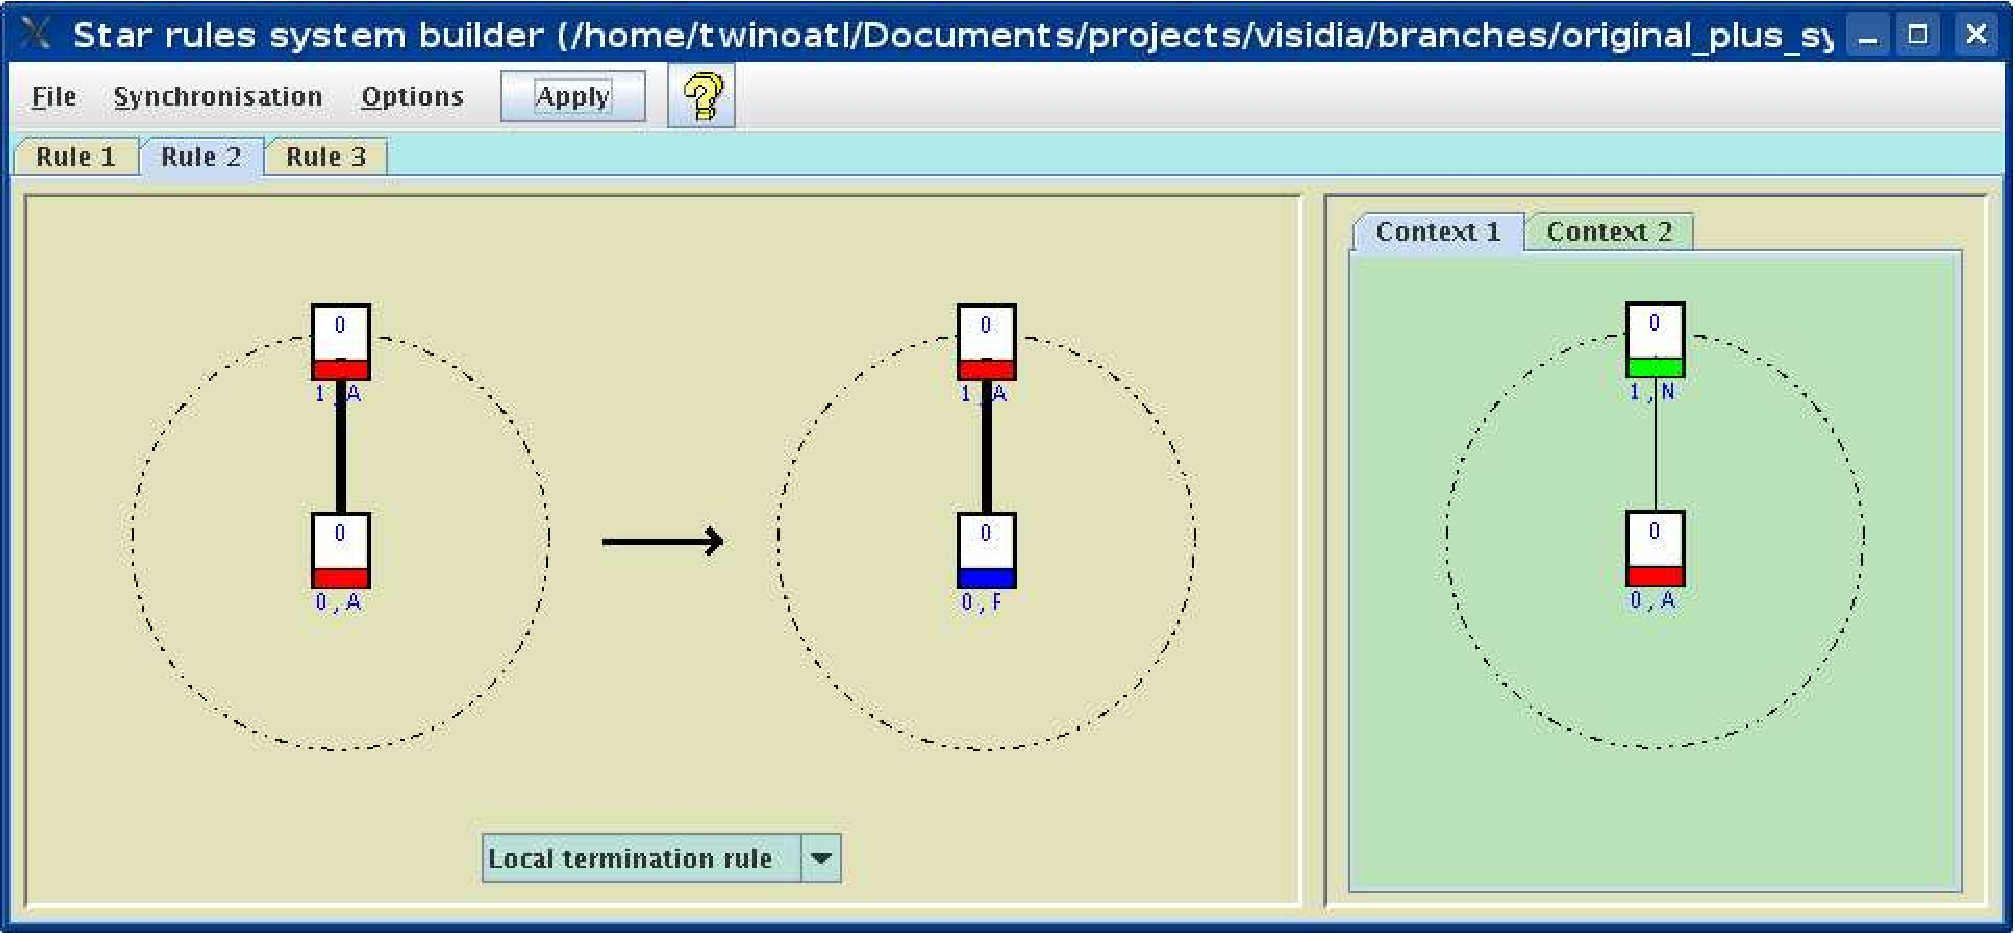
\includegraphics[width=14cm]{regles-reecritures}
  \caption{Les  r�gles de r��critures  sont implant�es  dans \visidia.
    L'utilisateur peut simplement  dessiner ses algorithmes.  Ici, est
    pr�sent�e   une   des  r�gles   de   r��critures  utilis�es   pour
    l'algorithme d'arbre recouvrant  avec d�tection de la terminaison.
    Cette r�gle dit: ``Si $u$ est  un sommet de label ``A'' qui a pour
    voisin un  sommet $v$  de label ``A''  aussi, que l'ar�te  qui les
    s�pare est marqu�e  (en gras) et que $u$ n'a pas  de voisin $w$ de
    label ``N'' avec une ar�te  non marqu�e (``Context 1''), alors $u$
    peut  prendre ``F''  comme label  (en r�alit�,  il y  a  une autre
    exclusion qui est cach�e sous l'onglet ``Context 2'')''.}
  \label{fig:existant-regles}
\end{figure}

\section{Ex�cution de la simulation}

Une  fois vos agents  en place,  vous pouvez  lancer la  simulation en
cliquant sur  le bouton start. Tous  les agents que  vous avez ajout�s
sur  le graphe  seront alors  lanc�s. Vous  pouvez  cependant toujours
influer sur le d�roulement de la simulation :

\begin{figure}[ht]
  \centering
  
\includegraphics[width=6cm]{boutons-exec}
  \caption{Les boutons pour influer  sur la simulation. Le bouton save
permet, lui, de sauvegarder le graphe courant}
  \label{fig:boutons-exec}
\end{figure}

\subsection{Bouton pause}

La simulation  se met en  pause le temps  que vous le souhaitez  : les
agents  et  le  simulateur  cessent  leurs  activit�s,  mais  existent
toujours.  Vous  avez donc  acc�s aux whiteboards  des sommets  et des
agents, ainsi qu'aux statistiques.\\

R�appuyez sur le bouton \textbf{pause} pour que la simulation reprenne.

\subsection{Bouton stop}

La simulation  est stopp�e  : contrairement au  bouton \textbf{pause},
une fois la simulation stopp�e,  vous ne pouvez plus la reprendre.  Le
simulateur  n'existe plus,  les agents  non plus,  il n'est  donc plus
possible  d'acc�der aux  whiteboards des  agents. Les  whiteboards des
sommets restent cependant accessibles, tout comme les statistiques.

\subsection{Bouton speed}

Ce  bouton  influence  la   vitesse  de  d�placement  des  agents  sur
l'interface graphique :  plus la vitesse est lente,  plus ils mettront
de temps � se d�placer d'un sommet � un autre.\\

\subsection{Bouton RESET}

Le   bouton   \textbf{RESET}  permet   de   remettre  l'ensemble   des
informations � z�ro (agents, whiteboards, statistiques, etc).  Si vous
venez de  lancer une  simulation et que  vous souhaitez en  lancer une
autre, vous devez au pr�alable utiliser le bouton reset : vous pourrez
alors de nouveau ajouter des agents sur le graphe.

\subsection{Pulse Counter}

En bas � droite de la fen�tre de simulation se trouve un champ ``Pulse
Counter''.   Celui-ci  est  d�gris�  lors  de  l'utilisation  d'agents
synchronis�s, et  correspond au nombre  de tops (ou  pulses) effectu�s
par les agents synchronis�s.\\

\begin{figure}[ht]
  \centering
  
\includegraphics[width=3cm]{pulse-counter}
  \caption{Le  champ  pulse counter  lors  d'une  simulation avec  des
  agents synchronis�s}
  \label{fig:pulse-counter}
\end{figure}

Pour plus de renseignements sur les pulses et les agents synchronis�s,
veuillez vous r�ferer � la section \ref{sec:prog-agent-synchro}.


\section{Utilisation des WhiteBoards}

Les whiteboards sont une particularit�  de la partie agent de \visidia
:  il s'agit simplement  d'un regroupement  d'informations li�es  � un
sommet ou � un agent.

\begin{figure}[ht]
  \centering
  
\includegraphics[width=5cm]{whiteboards}
  \caption{Les 3  icones d�di�es  � l'acc�s et  � la  modification des
  whiteboards,  dans   l'ordre  :  whiteboard  propre   �  un  sommet,
  whiteboard commun � tous les sommets, whiteboard propre � un agent}
  \label{fig:whiteboards-icons}
\end{figure}

\subsection{WhiteBoards des agents}

Chaque agent  poss�de un whiteboard pour y  stocker diverses variables
auxquelles il peut acc�der  en lecture et �criture. Concr�tement, cela
revient au m�me que de d�clarer des variables lors de la programmation
de  l'agent,  mais les  whiteboards  ont  l'avantage  de pouvoir  �tre
visualisables  en temps  r�el  lors d'une  simulation via  l'interface
graphique.   Ils  permettent de  plus  la  modification des  variables
durant la simulation par l'utilisateur.

Pour acc�der au whiteboard d'un agent, voici la manipulation � faire :
\begin{enumerate}
\item Cliquez sur le bouton ``agent whiteboard'' de l'interface.
\item  Choisir  l'agent dont  on  souhaite  consulter  ou modifier  le
whiteboard
\end{enumerate}

\begin{figure}[ht]
  \centering
  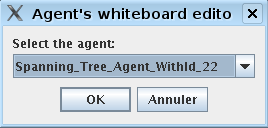
\includegraphics[width=5cm]{whiteboards-agent}
  \caption{Apr�s avoir cliqu� sur  l'icone whiteboard pour agent, vous
  devez  selectionner   l'agent  dont  vous   souhaitez  consulter  le
  whiteboard}
  \label{fig:whiteboards-agent}
\end{figure}

Pour savoir comment modifier le whiteboard d'un agent, consultez la section
\ref{sec:interface-whiteboards-modif}.

\subsection{WhiteBoards des sommets}

Comme pour  les agents, il est  possible de stocker  des variables sur
les  sommets en utilisant  des whiteboards  d�di�s �  �a. Ce  sont les
agents  qui   consultent  ou   modifient  ces  whiteboards,   ou  bien
directement l'utilisateur.\\

L'acc�s et la modification de valeurs se font de 2 fa�ons : 

\begin{itemize}

\item  En s�lectionnant  un sommet  (clic droit  de la  souris  sur le
sommet) puis  en cliquant  sur le bouton  ``info'' de  l'interface. De
cette mani�re on acc�de au whiteboard local au sommet s�lectionn�.

\item En  cliquant sur  le bouton ``initialize''  de l'interface  : on
acc�de alors  aux champs communs  � tous les sommets,  un ``whiteboard
global''. Cette action est surtout utile si l'on souhaite rajouter une
variable qui n'existe pas encore sur tous les sommets.

\end{itemize}

\begin{figure}[ht]
  \centering
  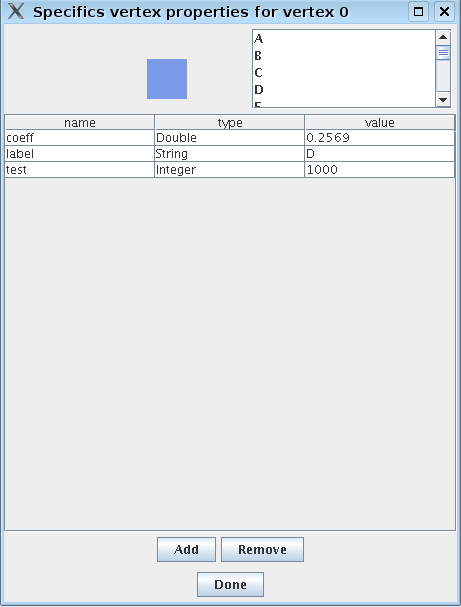
\includegraphics[width=9cm]{whiteboards-sommet}
  \caption{Apr�s  avoir s�lectionn�  un sommet  et cliqu�  sur l'icone
``info'', vous  acc�derez �  cette fen�tre. Vous  pouvez ici  voir les
variables  associ�es �  ce sommet,  les  modifier, en  ajouter, ou  en
supprimer. La fen�tre  de d�filement en haut �  droite est rattach�e �
la variable ``label''}
  \label{fig:whiteboards-sommet}
\end{figure}

Pour savoir comment modifier les valeurs de ces whiteboards, consultez
la section \ref{sec:interface-whiteboards-modif}.


\subsection{Modification des whiteboards}
\label{sec:interface-whiteboards-modif}

Nous   d�crirons   ici  la   modification   des  whiteboards   (ajout,
suppression,  modification de  variables). L'interface  �tant  la m�me
pour les whiteboards des sommets  et des agents, nous ne d�crirons ces
possibilit�s qu'une seule fois.\\

A partir d'ici, on consid�re qu'un whiteboard est ouvert via une des
m�thodes d�crites ci-dessus.

\subsubsection{Ajout d'une variable}

\begin{enumerate}
\item Cliquez sur le bouton \textbf{Add}
\item S�lectionnez le type de variables que vous souhaitez int�grer au
whiteboard (String, int, double, ...)
\item  Choisissez un  nom pour  votre  variable (attention  : si  vous
ajoutez une variable  qui porte le nom d'une  variable d�j� existante,
cette derni�re sera �cras�e)
\item  Entrez une valeur associ�e � votre nouvelle variable
\end{enumerate}

\begin{figure}[ht]
  \centering
  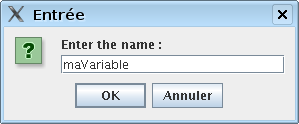
\includegraphics[width=6cm]{whiteboards-modif}
  \caption{Lorsque vous souhaitez ajouter  une variable, 3 �tapes sont
n�cessaires : choix du type de la variable, choix du nom puis choix de
sa valeur.}
  \label{fig:whiteboards-modif}
\end{figure}

\textbf{Cas particulier : } On consid�re que le whiteboard propre � un
sommet est  prioritaire par  rapport au whiteboard  global �  tous les
sommets. Ainsi, si  le nom d'une variable appara�t  en m�me temps dans
le  whiteboard global aux  sommets et  dans le  whiteboard local  � un
sommet, c'est cette  derni�re qui sera privil�gi�e. Ainsi  si un agent
demande la valeur de cette variable, ce sera la valeur locale qui sera
retourn�e.

\subsubsection{Suppression d'une variable}

\begin{enumerate}
\item S�lectionnez la variable � supprimer
\item Cliquez sur le bouton \textbf{Remove}
\end{enumerate}

\subsubsection{Modification d'une variable}

\begin{enumerate}
\item Cliquez sur le champ � modifier
\item Entrez la nouvelle valeur
\item Appuyez  sur ENTREE  pour que la  nouvelle valeur soit  prise en
compte
\end{enumerate}

\textbf{Cas particulier  :} Si vous  souhaitez modifier le  label d'un
sommet,  vous devez  utiliser la  liste  d�roulante situ�e  en haut  �
droite des whiteboards locaux des sommets.


\section{Visualisation des statistiques}

L'utilisation des statistiques  est un peu particuli�re :  on peut les
visualiser pendant  une simulation classique,  avec les agents  qui se
d�placent de mani�re visible sur le  graphe, mais on peut aussi ne pas
lancer la simulation graphique et uniquement voir les statistiques.

\begin{figure}[ht]
  \centering
  
\includegraphics[width=3cm]{statistics-button}
  \caption{Le bouton Statistics se  d�grise d�s l'ajout d'un agent sur
  le graphe}
  \label{fig:statistics-button}
\end{figure}

\subsection{Lancement pendant la simulation}

Vous pouvez  consulter les statistiques en plein  milieu de simulation
si vous le souhaitez : pour cela, vous devrez placer des agents sur le
graphe  puis lancer une  simulation comme  expliqu� dans  les sections
pr�c�dentes, puis cliquer sur le bouton \textbf{Statistics}.

\begin{figure}[ht]
  \centering
  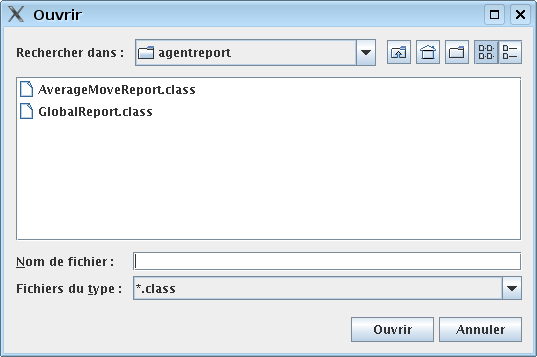
\includegraphics[width=11cm]{statistics-algo}
  \caption{Apr�s  avoir  cliqu�  sur  Statistics, vous  devez  choisir
quelles statistiques vous voulez afficher}
  \label{fig:statistics-algo}
\end{figure}

Apr�s avoir  cliqu� sur le bouton Statistics,  vous devez s�lectionner
la classe  de statistiques que vous  souhaitez. En effet,  il vous est
permis  de choisir  quelles statistiques  seront affich�es  et comment
elles seront  calcul�es. Par  exemple, vous pouvez  choisir d'afficher
toutes les statistiques, ou bien uniquement les statistiques li�es aux
d�placements, ou bien encore une  moyenne des d�placements de tous les
agents.    

Pour  savoir  comment  cr�er  ses  propres  classes  de  statistiques,
r�ferez-vous   �    la   section   \ref{sec:prog-stats}.\\

\begin{figure}[ht]
  \centering
  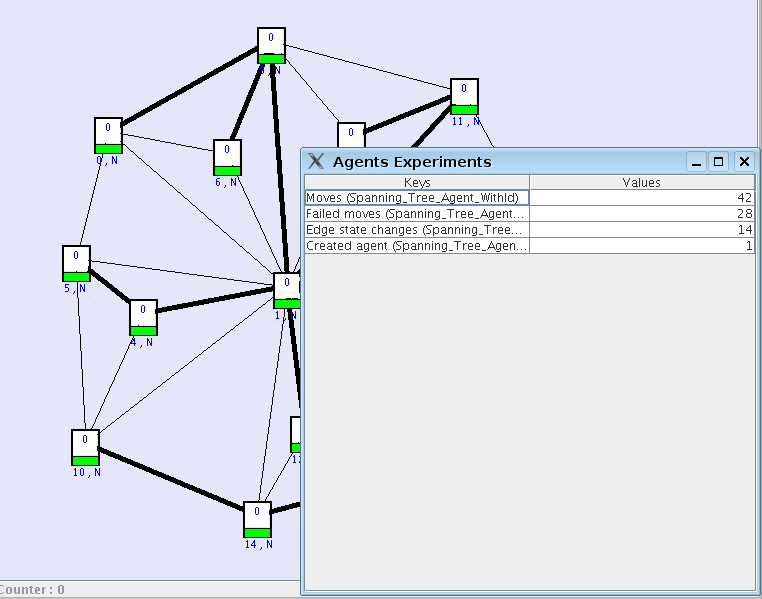
\includegraphics[width=13cm]{statistics-avec-simu}
  \caption{Un exemple  d'affichage de statistiques  avec la simulation
graphique lanc�e}
  \label{fig:statistics-avec-simu}
\end{figure}

Une fois  la classe choisie,  les statistiques s'afficheront  en temps
r��l,  et les  d�placements des  agents seront  toujours  visibles sur
l'interface graphique.

\subsection{Lancement en dehors d'une simulation}

Si voir les agents se d�placer graphiquement ne vous int�resse pas, et
que  vous d�sirez  une simulation  beaucoup plus  rapide,  vous pouvez
visualiser les statistiques sans lancer la simulation graphique.\\

Avant cela,  vous devez tout  de m�me dans  un premier temps  cr�er ou
charger  votre graphe,  puis placer  des agents  dessus comme  si vous
alliez lancer  une simulation graphique.  Une fois  cela fait, cliquez
sur le  bouton \textbf{Statistics}.  Puis, choisissez  votre classe de
statistiques comme expliqu� dans la section pr�c�dente.

\begin{figure}[ht]
  \centering
  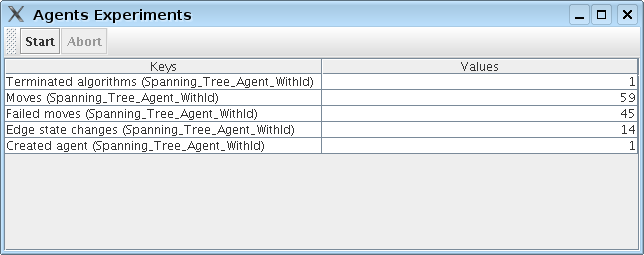
\includegraphics[width=13cm]{statistics-sans-simu}
  \caption{Un exemple  de statistiques sans  simulation graphique. Des
boutons \textbf{Start}  et \textbf{Abort} sont  apparus, correspondant
au d�marrage et � l'arr�t de la simulation}
  \label{fig:statistics-sans-simu}
\end{figure}

Vous pouvez alors cliquer  sur le bouton \textbf{Start} pour commencer
la simulation : vous verrez  les statistiques �voluer, mais les agents
resteront  fig�s sur  le  graphe.  Pour mettre  fin  � la  simulation,
cliquez simplement sur le bouton \textbf{Abort}.

%%% Local Variables: 
%%% mode: latex
%%% TeX-master: "main"
%%% coding: latin-1
%%% TeX-PDF-mode: t
%%% End: 

\chapter{Programmer des agents avec l'API}

% mini-plan de la section
% Programmation      
%   Agent
%   Agent Sync
%   Mover
%   Placeur
%   Stats

Dans cette section, nous commencerons par voir l'API de programmation
des agents puis la m�thode � adopter pour en programmer de
nouveaux. Nous verons �galement comment programmer des algorithmes de
d�placement, avant de nous interreser � l'implantation de techniques de
placement initial d'agents. Et pour conclure nous verrons comment il
est possible de cr�er des statistiques persnnalis�es.\\

Vous pouvez aussi vous baser sur des exemples d�j� �crits ; vous en
trouverez un grand nombre dans les r�pertoires :
\begin{itemize}
\item \dossier{sources/visidia/agents} pour les agents.
\item \dossier{sources/visidia/agents/agentsmover} pour les algorithmes de d�placement.
\item \dossier{sources/visidia/agents/agentchooser} pour le placement
  initial d'agents.
\item \dossier{sources/visidia/agents/agentreport} pour la creation de
  statistiques.
\end{itemize}


\section{Description de l'API}
\label{sec:agent-api}

Toute la documentation a �t�  �crite � l'aide de Javadoc. Pour g�n�rer
des fichiers  HTML, placez vous  dans le dossier  \dossier{visidia} et
tapez la commande suivante :

\begin{verbatim}
$ ./mkjavadoc.sh
$
\end{verbatim}

Ceci  fait, ouvrez le  fichier \dossier{visidia/javadoc/index.html}
avec un navigateur puis s�lectionnez la classe Agent. 


\section{Ecrire ses propres agents}

Il existe deux types d'agents : les agents non-synchronis�s et les
agents synchronis�s.

Dans ces deux cas, vous devez cr�er respectivement une sous-classe de la classe
\classe{Agent} ou de la classe \classe{SynchronizedAgent} et la placer
dans le dossier \dossier{visidia/sources/visidia/agents}.  N'oubliez
pas de renseigner le package gr�ce � la ligne :

\begin{verbatim}
package visidia.agents;
\end{verbatim}

La programmation de l'agent se fait en impl�mentant la
m�thode \methode{init()} et en utilisant les diff�rentes possibilit�s
offertes par l'API.\\


\subsection{Cas d'un agent non-synchronis�}

\begin{verbatim}

  protected void init() {
      
    do {
      Integer nbPassages;

      try {
        nbPassages = (Integer) getVertexProperty("nbPassages");
      } catch (NoSuchElementException e) {
        nbPassages = 0;
      }

      nbPassages = new Integer(nbPassages.intValue() + 1);
      setVertexProperty("nbPassages", nbPassages);

      Random rand = new Random();

      moveToDoor(rand.nextInt(getArity()));
    } while (true);
  }
\end{verbatim}

L'objectif de cet agent est de compter le nombre de passage des agents
sur chaque sommet.  Pour m�moriser le nombre de passage sur chaque
sommet, nous avons utilis� le champs ``nbPassages'' du whiteboard du
sommet.

Pour ce faire, nous essayons dans un premier temps de r�cup�rer le
nombre de passages de ce type d'agent sur le whiteboard du sommet
courant par le biais de la
\methode{getVertexProperty(``nbPassages'')}. Si ce champs n'a pas �t�
pr�alablement inscrit dans le whiteboard du sommet, l'appel � la
m�thode \methode{getVertexProperty(``nbPassages'')} va d�clencher une
exception de type \emph{NoSuchElementException}. Si tel est le cas,
nous consid�rons qu'il s'agit de notre premier passage. Ceci est
effectu� dans le \emph{catch}.

Ensuite, nous incr�mentons le nombre de passages de un, puis l'agent
r��crit la nouvelle valeur dans le champs ``nbPassages'' du sommet
courant gra�e � la m�thode \methode{setVertexProperty(``nbPassages'')}.

\subsection{Cas d'un agent synchronis�}
\label{sec:prog-agent-synchro}

\begin{verbatim}
public class BasicSynchronizedAgent1 extends SynchronizedAgent {

    protected void init() {

        for(int i=0; i<10; ++i) {
          Random rand = new Random();
	 
          nextPulse();
          moveToDoor(rand.nextInt(getArity()));

        }

    }
}
\end{verbatim}

Cet agent se d�place al�atoirement � travers le graphe et meurt au
bout de 10 d�placements. Veuillez noter l'appel � la m�thode
\methode{nextPulse()} qui permet de synchroniser les agents : chaque
agent synchronis� sera bloqu� � l'appel de cette m�thode jusqu'� ce
que le dernier agent synchronis� fasse � son tour appel � cette
m�thode. Un rendez-vous, c'est � dire une rencontre entre agents, peut
alors �tre organis�.

Le rendez-vous est r�alis� en impl�mentant la m�thode
\methode{planning(SynchronizedAgent)} qui sera appel� � chaque fois
qu'un rendez-vous � lieu sur un sommet.


\section{D�velopper des algorithmes de d�placement}

La m�thode de cr�ation d'algorithmes de d�placement est presque
identique � la m�thode de cr�ation d'agents. Pour cela il suffit de
sous classer la classe \classe{AgentMover} et implanter la m�thode
\methode{findNextDoor()}. De plus vous disposez de toutes les
informations n�cessaires sur l'agent gr�ce � la m�thode
\methode{agent()}.  Les algorithmes que vous �crirez devront se
trouver dans le paquet \dossier{visidia.agents.agentsmover}.



Voici le code d'un algorithme d'un d�placement al�atoire :

\begin{verbatim}
public class RandomAgentMover extends AgentMover {
    
    public RandomAgentMover(Agent ag) {
        super(ag);
    }

    protected int findNextDoor() {
        Random rand = new Random();

        return rand.nextInt(agent().getArity());
    }
}
\end{verbatim}

Pour utiliser cet algorithme de d�placement pour un agent, utilisez le
m�thode \methode{setAgentMover(``RandomAgentMover'')} . Le nom pass�
en param�tre doit correspondre exactement au nom de la classe (casse
comprise). Le d�placement ne se fera plus avec
\methode{moveToDoor(int)} mais avec \methode{move()}

Voici comment nous pouvons r��crire notre BasicSynchronizedAgent1 :

\begin{verbatim}
public class BasicSynchronizedAgent1 extends SynchronizedAgent {

  protected void init() {
    setAgentMover("RandomAgentMover");
    
    for(int i=0; i<10; ++i) {
      
      nextPulse();
      move();
    }
}
\end{verbatim}

Pour plus d'informations, r�f�rez vous � la javadoc comme indiqu� en
\ref{sec:agent-api} et lisez particuli�rement la documentation de la
classe \classe{AgentMover}.

D'autre exemples d'algorithmes de placement sont disponibles dans le
package \dossier{visidia.agents.agentsmover}

\section{Implanter des techniques de placement initial d'agents}
\label{sec:prog-placeur}

Comme pour les algorithmes de d�placement des agents sur le graphe, la
programmation  de nouveaux  algorithmes de  placement d'agent  se fait
simplement   et  la  lecture   de  la   documentation  de   la  classe
\classe{AgentChooser}  ainsi  que  le  parcours des  exemples  devrait
suffire.\\

Vos algorithmes de placement d'agents devront �tre implant�s dans le
paquet \dossier{visidia.agents.agentchooser}, devront surcharger la
m�thode \methode{chooseForVertex(Integer)} et devront appeler la
m�thode \methode{addAgent(Integer, String)} pour ajouter des agents.



\section{Cr�ation de statistiques personnalis�es}
\label{sec:prog-stats}

La cr�ation de statistiques peut etre enti�rement personnalis�e.  Pour
cela il vous faudra �crire une classe h�ritant de
\classe{AbstractStatReport} dans laquelle vous devrez red�finir la
m�thode \methode{getStats()} qui retournera l'ensemble des
statistiques.  Ces statistiques devront faire partie du package
\dossier{visidia.agents.agentreport}

Voici un exemple calculant le nombre de d�placements moyen par type
d'agent :

\begin{verbatim}
public class AverageMoveReport extends AbstractStatReport {
    /**
     * Used to store the number of agents of type given by Class. Keys
     * represent the class of agents (BasicAgent, SpanningTree...) and
     * values represent the number of agents for that class.
     */
    private Hashtable<Class, Long> agentsByClass;

    /**
     * Will  store the  report  information. Everything  that will  be
     * displayed on the report will be in that variable.
     */
    private Bag stats;

    /**
     * Used to fill the <code>agentsByClass</code> instance variable.
     */
    private void countAgents() {
	Set keys;
	agentsByClass = new Hashtable(10);

	/**
	 * Keys is  a Set  containing all the  events reported  by the
	 * simulator.
	 */
	keys = getBag().keySet();

	/**
	 * For each events
	 */
	for(Object key: keys) {
	    if (key instanceof AgentCreationStat) // if    it   is   a
						  // creation event
		agentsByClass.put(((AgentCreationStat)key).getAgentClass(),
				  new Long(getBag().getOccurrencesOf(key)));
	}
    }

    /**
     * Count the moves by agent type.
     */
    private void computeStats() {
	Set keys;

	stats = new Bag();

	countAgents();

	/**
	 * Keys is a set containing all the events.
	 */
	keys = getBag().keySet();

	for(Object key: keys) {
	    float movesByAgent;

	    if (key instanceof MoveStat) { // if it is a move event
		Class agClass = ((MoveStat)key).getAgentClass();
		long agentsForClass = agentsByClass.get(agClass).longValue();
		long movesForClass = getBag().getOccurrencesOf(key);

		stats.add("Average moves by agent (" 
			  + agClass.getSimpleName() + ")",
			  new Long(movesForClass / agentsForClass));
	    }
	}
    }

    /**
     * Calculate the  number of  moves by agent  type and  returns the
     * results that will be displayed.
     */
    public Bag getStats() {
        computeStats();
        return stats;
    }

\end{verbatim}


\end{document}

%%% Local Variables: 
%%% mode: latex
%%% TeX-master: "main"
%%% coding: latin-1
%%% TeX-PDF-mode: t
%%% End: 

%%% Local Variables: 
%%% mode: latex
%%% TeX-master: t
%%% coding: latin-1
%%% TeX-PDF-mode: t
%%% End: 
